\documentclass[../SWD_disp.tex]{subfiles}

\begin{document}
\section{Observer Pattern}

Giv definitionen af et design pattern til at starte med.

\subsection{Opbygning af Observer Pattern}
Observer Pattern er i gruppen af behavioral patterns, fordi den denfinerer måden for kommunkationen mellem klasserne.
\\

Det tillate et enkelt object kendt som "subject" til, at publiserer ændringer i dens state. En eller mange observer objekter der afhænger af subjects, kan subscribe til et, således at de automatisk bliver notificeret.
\\

Observer Pattern giver lav koblint mellem subjects og observers
\\

Provider (data der ændres) og Consumer (data der skal hentes fra provider)
\begin{itemize}
    \item Vi skal kunne tillate consumeren til at blive tilføjet (attached) til provideren uden, at ændre implementeringsmæssigt for Procider (OCP)
    \item Tillade provideren til at informaerer consumers ved data ændring (lav kobling)
    \item Tillage mange consumers til, at blive informeret på opdatering af den samme data.
    \item Se efter 1-many afhængigheder således, at når det ene object ændrer state, til dens afhængige blive notificeret og opdateret automatisk.
\end{itemize}

\begin{figure}[H]
    \centering
    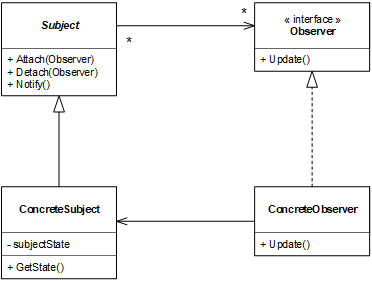
\includegraphics{observer_pattern.PNG}
    \caption{Observer Pattern}
    \label{fig:observer_pattern}
\end{figure}

At anvende SOLID principper, fremmer godt software design. at følge OCP betyder at du får lav kobling mellem dine klasser. Dette resultere yderemere i software som er let at teste.

\subsection*{Fordele}
\begin{itemize}
    \item Skaber lav kobling mellem provider og consumer objekter.
    \item Tillader ét subject at opdateren x antal observers automatisk. 
    \item Ingen behov for, at modificerer på Subject ved tilføjelse af nye observers. Dette er pga. OCP.
    \item Tilføje og fjerne eksisterende observers til enhver tid.
\end{itemize}

\subsection*{Ulemper}
\begin{itemize}
    \item Rækkefølgen af notifications af observers kan være uafhængig.
    \item Memoryleak kan forekomme i ikke Garbage-Collection sprog pga. du explicit skal attach og detach Subject.
\end{itemize}
\subsection{Push vs Pull Observer}
donger


% \subsection*{Forskellige varianter af GoF Observer}
% \subsubsection*{Subject af samme type}
% \begin{figure}[H]
%     \centering
%     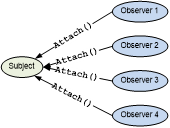
\includegraphics[scale = 1.5]{subject_same_type.PNG}
%     \caption{Subject Same Type}
%     \label{fig:subject_same_type}
% \end{figure}


% \subsubsection*{Ved samme type implementering}
% \begin{figure}[H]
%     \centering
%     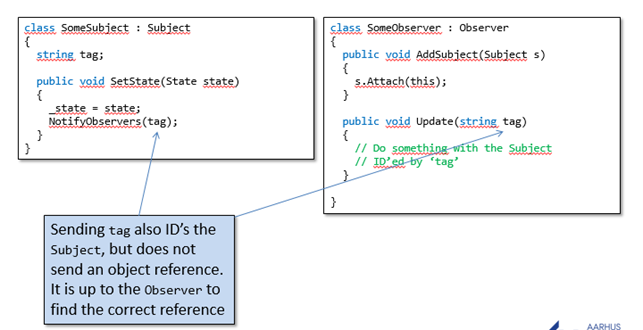
\includegraphics{same_type_impl.PNG}
%     \caption{Samme Type Implementering}
%     \label{fig:same_type_impl}
% \end{figure}

% \subsubsection*{Ved håndtering af subjekt af forskellige typer:}
% \begin{figure}[H]
%     \centering
%     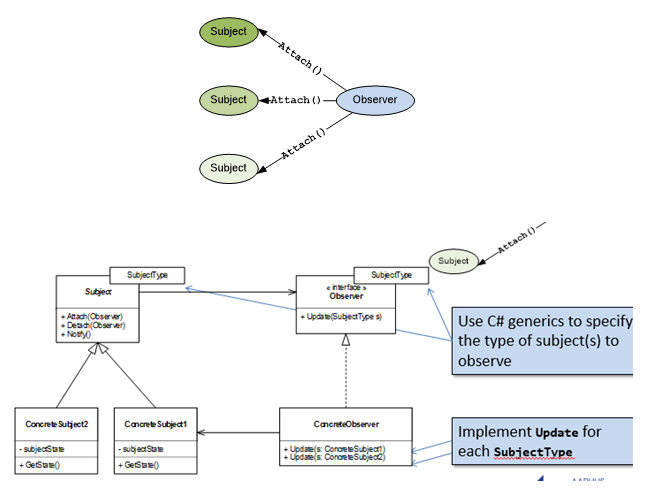
\includegraphics{subject_different_type.PNG}
%     \caption{Subject af forskellige typer}
%     \label{fig:subject_diff_type}
% \end{figure}
\end{document}
